\chapter{Исследовательская часть}

\section{Технические характеристики}

Технические характеристики устройства, на котором выполнялось исследование представлены далее:
\begin{enumerate}[label=\arabic*)]
	\item операционная система Ubuntu 22.04.3~\cite{ubuntu};
	\item процессор \textit{Intel Core i5-1135G7} 2.4 ГГц;
	\item оперативная память 16 ГБ, \textit{DDR4}.
\end{enumerate}

Во время исследования времени ноутбук был нагружен только встроенными приложениями окружения, не был включен в сеть питания.

\section{Описание исследования}

Целью экперимента является исследование зависимости времени выполнения запроса к таблице базы данных при разном количестве записей в ней. А так же необходимо провести сравнительный анализ при наличии индекса в этой таблице и без него.

Для исследования использовалась таблица \textit{Schedules}, так как чаще всего и клиентам, и тренерам требуется посмотреть расписание тренировок.

Индекс создавался на поле \textit{date\_and\_time} с помощью следующей команды

\begin{lstlisting}
CREATE INDEX IF NOT EXISTS IX_Schedules_DateAndTime ON public."Schedules" (date_and_time)
\end{lstlisting}

Замеры проводились для разного количества записей в таблице: от 10 до 5000. Так же при каждом количестве время замерялось по 100 раз и после этого усреднялось.
\clearpage

\section{Результаты исследования}

Результаты замеров приведены в таблице \ref{tbl:time_mes} (время в мс.).
 
\begin{table}[h]
	\begin{center}
		\begin{threeparttable}
			\captionsetup{singlelinecheck=off, justification=raggedright}
			\caption{Результаты замеров времени}
			\label{tbl:time_mes}
			\begin{tabular}{|c|r|r|}
				\hline
				Количество записей & Время без индекса & Время с индексом \\ 
				\hline
				10 & 0.001683 & 0.001860 \\ \hline
				100 & 0.010538 & 0.011872 \\ \hline
				250 & 0.030085 & 0.025258 \\ \hline
				500 & 0.070169 & 0.049925 \\ \hline
				1000 & 0.199291 & 0.112767 \\ \hline
				1500 & 0.361543 & 0.150151 \\ \hline
				2000 & 0.565231 & 0.203894 \\ \hline
				2500 & 0.743195 & 0.258923 \\ \hline
				3000 & 0.988928 & 0.332711 \\ \hline
				3500 & 1.582918 & 0.400369 \\ \hline
				4000 & 1.937912 & 0.453513 \\ \hline
				5000 & 2.363422 & 0.576650 \\ \hline
			\end{tabular}
		\end{threeparttable}
	\end{center}
\end{table}

Также на рисунке \ref{fig:graph} приведены графические результаты замеров времени выполнения запроса.

\clearpage

\begin{figure}[h!]
	\centering
	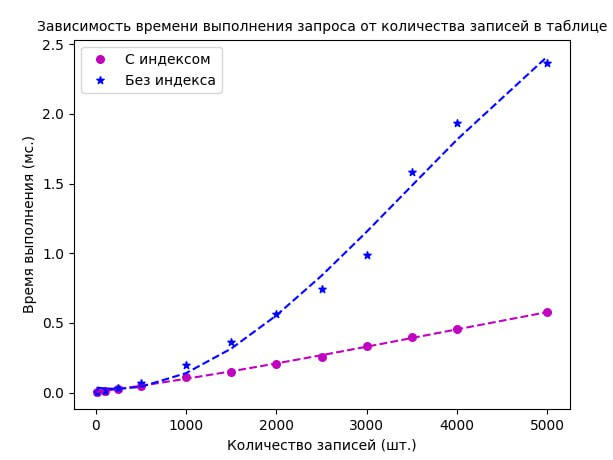
\includegraphics[width=\linewidth]{img/graph}
	\caption{Сравнение по времени выполнения запроса от количества записей в таблице с использованием индекса и без него}
	\label{fig:graph}
\end{figure}

\section*{Выводы к исследовательской части}

В данной части был проведен сравнительный анализ времени выполнения запроса к таблице базы данных для получения записей из расписания в конкретный день. Из проведенного эксперимента можно сделать вывод, что функция зависимости времени без использования индекса растет быстрее, чем с ним.

При количестве записей менее 250 время выполнения запроса без индекса меньше, чем с индексом, но при большем количестве запрос без использования индекса выполняется дольше. Причем чем больше количество записей, тем сильнее растет разница во времени. Так при количестве записей в таблице, равном 500, отношение времен между рассматриваемыми вариантами составляет 1.4 раза, а при количестве записей, равном 5000, уже 4.1 раза.
